\chapter{Resultados y Discusión}
\label{resultadosdiscusion}
\ifpdf
  \graphicspath{{Chapter6/Chapter6Figs/PNG/}{Chapter6/Chapter6Figs/PDF/}{Chapter6/Chapter6Figs/}}
\else
  \graphicspath{{Chapter6/Chapter6Figs/EPS/}{Chapter6/Chapter6Figs/}}
\fi

\markboth{\hfill \thechapter. Resultados y Discusión}{\hfill \thechapter. Resultados y Discusión}

\section{Ambiente de Ejecución.}

Para la ejecución del proceso de optimización se utilizaron equipos con la siguiente configuración:
\begin{itemize}
\item Una computadora de escritorio con procesador Intel Core i5 de cuatro núcleos, con 8 GB de memoria RAM, y sistema operativo Windows 7 de 64 bits.
\item Una computadora de escritorio con procesador Intel Core i5 de cuatro núcleos, con 4 GB de memoria RAM, y sistema operativo Windows 7 de 64 bits.
\end{itemize}

Para la implementación del \textit{SMPSO-CLAHE}, se utilizaron librerías libres disponibles en la web. La implementación de la metaheurística \textit{PSO multi-objetivo} se encuentra escrita en el lenguaje JAVA, es una adaptación de la implementación original planteada y disponible en las librerías $jMetal$ \cite{Durillo2011}. Fue modificada para computar el cálculo del $fitness$, basándonos en que se desea maximizar la cantidad de información de la imagen y minimizar la distorsión de la misma.

Para la implementación del algoritmo \textit{CLAHE} y las métricas de evaluación, Entropía (\ref{sec:entropia}), Entropía Local (\ref{sec:entropialocal}), \textit{SSIM} (\ref{sec:ssim}) y \textit{LTG} (\ref{sec:ltg}), se toman como base las implementaciones existentes en \textit{Matlab} \cite{MatlabOTB}. 

Para la interoperabilidad entre las implementaciones del \textit{SMPSO multi-objetivo}, $CLAHE$ y las métricas de evaluación, se utilizó un esquema de intercambio de mensajes via socket (TCP/IP Socket Communications). 

Las pruebas se realizaron empleando 30 imágenes radiológicas previamente digitalizadas del tórax obtenidas del sitio https://openi.nlm.nih.gov/. Las mismas se seleccionaron a partir de la cantidad de detalles que poseen, lo que representa un desafío adecuado para la {\it mejora del contraste}.

Se realizaron 30 ejecuciones de \textit{SMPSO-CLAHE} por cada imagen de prueba, con un tamaño de enjambre de 70 partículas y el tamaño del archivo de líderes fue de 70. Se obtuvieron aproximadamente 300 imágenes soluciones Pareto por cada una de ellas, las cuales fueron nuevamente filtradas una vez terminadas las ejecuciones.


\section{Resultados Obtenidos.}

Los resultados experimentales obtenidos de las correlaciones entre los pares de métricas utilizados se muestran en las \textbf{Tablas \ref{tabla:correlacionFrontal} y \ref{tabla:correlacionLateral}} , donde los valores marcados en negrita demuestran la fuerte relación inversa lineal existente entre los pares de métricas, lo cual indica que estas métricas se complementan para mantener el compromiso entre aumento de contraste y minimización de la distorsión. El {\it coeficiente de correlación de Pearson}, obtenido a través de los coeficientes de las funciones objetivo durante las pruebas, muestra el comportamiento en términos de cuánto una métrica afecta a la otra debido al proceso de {\it mejora del contraste}.

\begin{table}[H]
\begin{center}
\caption{Resultados de promediar la correlación de Pearson usando Entropía ($\mathscr{H}$), Entropía Local ($\mathscr E$), \textit{SSIM} y \textit{LTG}, para imágenes de tórax frontal.}
 \begin{tabular}{|c|c|c|c|c|}
            \hline
            Métricas & $\mathscr{H}$ & $\mathscr{E}$ & \textit{SSIM}\\
            \hline
            $\mathscr{E}$ & -0.83918  &  &  \\ \hline
            \textit{SSIM} & -0.84739 & \textbf{-0.97740} & \\ \hline
            \textit{LTG} & -0.81365 & -0.96307 &  0.00923   \\ \hline
            \end{tabular}
\label{tabla:correlacionFrontal}
\end{center}
\end{table}

\begin{table}[H]
\begin{center}
\caption{Resultados de promediar la correlación de Pearson usando Entropía ($\mathscr{H}$), Entropía Local ($\mathscr E$), \textit{SSIM} y \textit{LTG}, para imágenes de tórax lateral.}
\begin{tabular}{|c|c|c|c|c|}
            \hline
            Métricas & $\mathscr{H}$ & $\mathscr{E}$ & \textit{SSIM} \\
            \hline
            $\mathscr{E}$ & -0.24288  &  &   \\ \hline
            \textit{SSIM} & -0.79984 & \textbf{-0.95521} &  \\ \hline
            \textit{LTG} & -0.39579 & -0.84976 & 0.33629    \\ \hline
            \end{tabular}
\label{tabla:correlacionLateral}
\end{center}
\end{table}

De acuerdo a los resultados obtenidos en la correlación de Pearson, se determina la fuerza de las relaciones entre las métricas \textit{Entropía Local} y \textit{SSIM}, ambas métricas demuestran ser las más contradictorias. Esto no significa que las demás métricas no sean contradictorias, simplemente optamos por el mayor valor de contradicción, según la correlación obtenida, que son el par de métricas \textit{Entropía Local} ($\mathscr{E}$) e \textit{Índice de Similitud Estructural} (\textit{SSIM}), esto indica que el mejoramiento de una función objetivo es logrado a costa del empeoramiento de la otra función objetivo en un contexto de minimización o maximización de ambas.

Se utilizó la correlación de Pearson para medir el grado de relación  de los pares de métricas, que fueron utilizados como funciones objetivos en el proceso de optimización Robusta.


En la \textbf{Figura  \ref{fig:resultado_entropia_local_ssim_img1}} se muestran las soluciones obtenidas correspondientes a una imagen de tórax frontal y en la \textbf{Figura  \ref{fig:resultado_entropia_local_ssim_img9}} se muestran las soluciones obtenidas correspondientes a una imagen de tórax lateral, que se encuentran en el Conjunto Pareto para las métricas {\it Entropía Local/SSIM}, además de la imágenes originales como referencia visual.

%Imagen 1 torax frontal entropia local/ssim
\begin{figure}[H]
    \begin{center}
        \subfigure[][\label{fig:label:a} $SSIM=1$ \space $\mathscr{E}=3.4754$
        ]{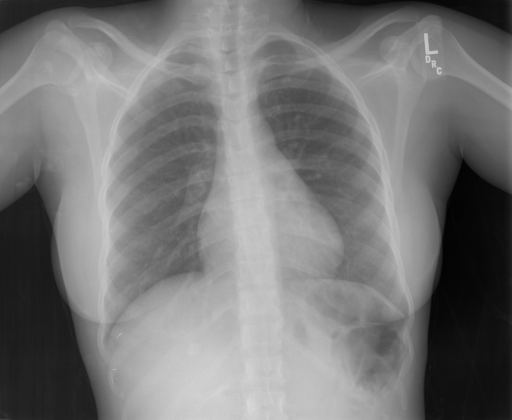
\includegraphics[width=4.5cm]{entropia_local_ssim/imagen1.png}}
        \subfigure[][\label{fig:label:b} $SSIM=0.7402$ \space $\mathscr{E}=4.5639$]{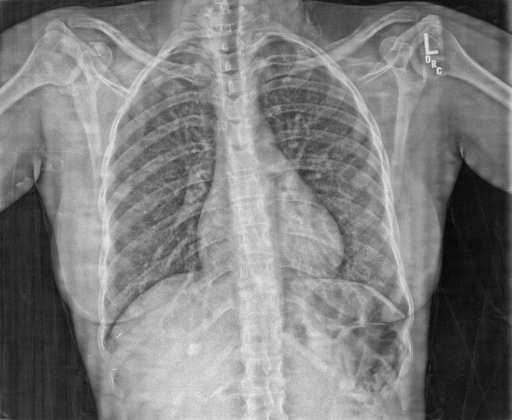
\includegraphics[width=4.5cm]{entropia_local_ssim/imagen1_193_41_0_local_ssim.png}}
        \subfigure[][\label{fig:label:c} $SSIM=0.9724$ \space  $\mathscr{E}=3.8264$]{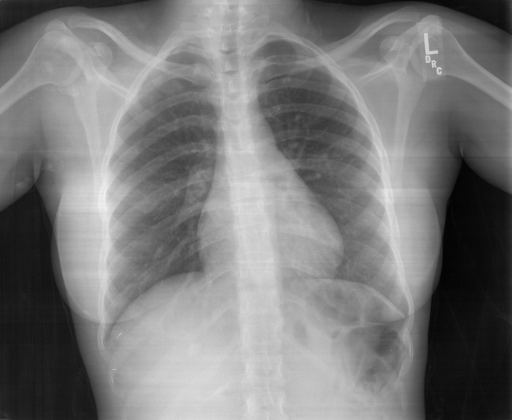
\includegraphics[width=4.5cm]{entropia_local_ssim/imagen1_210_3_0_local_ssim.png}}
    \end{center}
    \caption{Tórax frontal 1.}
    \captionsetup{aboveskip=0pt}
    \caption*{ Imagen Original \ref{fig:label:a}, Imágenes resultantes \ref{fig:label:b} y \ref{fig:label:c}}
    \label{fig:resultado_entropia_local_ssim_img1}
\end{figure}

%Imagen 9 torax lateral entropia local/ssim
\begin{figure}[hbtp]
    \begin{center}
        \subfigure[][\label{fig:label:d} $SSIM = 1$ \space $\mathscr{E}=2.8157$
        ]{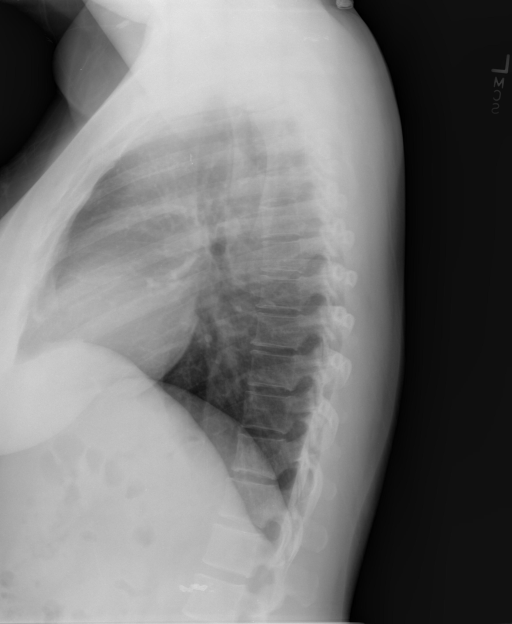
\includegraphics[width=4.5cm]{entropia_local_ssim/imagen9.png}}
        \subfigure[][\label{fig:label:e} $SSIM=0.8871$ $\mathscr{E}=3.4791$]{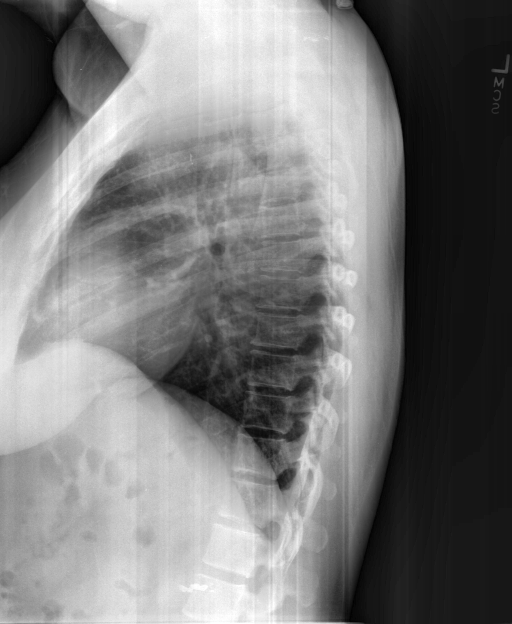
\includegraphics[width=4.5cm]{entropia_local_ssim/imagen9_2_256_0-005186957854_local_ssim.png}}
        \subfigure[][\label{fig:label:f} $SSIM=0.9016$ $\mathscr{E}=3.4296$]{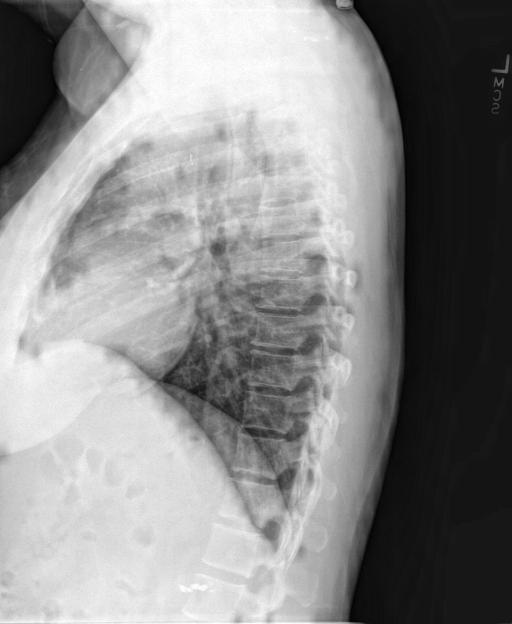
\includegraphics[width=4.5cm]{entropia_local_ssim/imagen9_49_82_0_local_ssim.png}}
    \end{center}
    \caption{Tórax lateral 2.}
    \captionsetup{aboveskip=0pt}
    \caption*{ Imagen Original \ref{fig:label:d}, Imágenes resultantes \ref{fig:label:e} y \ref{fig:label:f}}
    \label{fig:resultado_entropia_local_ssim_img9}
\end{figure}

La relación inversa entre las métricas se refleja en los resultados obtenidos. A partir de las Figuras \ref{fig:label:c} y \ref{fig:label:f} se observa que a medida que la métrica {\it SSIM} se aproxima a \textbf{1} los resultados se asemejan más a las imágenes originales, Figuras \ref{fig:label:a} y \ref{fig:label:d}, en términos de contraste, y de visibilidad de detalles; en cambio, mientras la {\it Entropía Local} aumenta se diferencian más los detalles no visibles debido al bajo contraste, Figuras \ref{fig:label:b} y \ref{fig:label:e}. 

Las imágenes que conforman el Conjunto Pareto resaltan distintos detalles a medida que los objetivos varían, lo cual se logra a partir de que se asegura la selección de las métricas más adecuadas para la optimización, basada en el análisis descrito anteriormente.

Las imágenes se dividieron en dos grupos, el primer grupo, imágenes de tórax lateral y el segundo grupo, imágenes de tórax frontal.

Se analizó el comportamiento del Conjunto Pareto resultante de cada imagen procesada, se consideró el {\it Frente Pareto óptimo} de una imagen $f$, como el conjunto de variables de decisión de las {\it N-1} imágenes y se obtuvo un nuevo {\it Frente Pareto} para las {\it N-1} imágenes. También se consideró como una sola entrada el conjunto de todas las imágenes y se realizó el cálculo de la Entropía Local \ref{sec:entropialocal} y SSIM \ref{sec:ssim} entre todas las imágenes de entrada; obteniendo así el {\it Frente Pareto Robusto}. De esta forma podemos observar si los valores del {\it Frente Pareto} de la imagen $f$ varían de forma significativa usando como entrada otras imágenes o son óptimas para las imágenes de referencia del mismo grupo.

% En la \textbf{Figura \ref{fp-original-resultante-tf}} se muestran el {\it Frente Pareto} óptimo de la imagen \textbf{\ref{fig:label:a}} y los Frentes Pareto sub-óptimos al variar las variables de decisión, tomando los Frentes Paretos de las otras imágenes del grupo. Se puede observar que algunos Frentes Pareto se desplazan con respecto al original.

En la \textbf{Figura \ref{fp-original-resultante-tf}} se muestran el {\it Frente Pareto} óptimo de la imagen \textbf{\ref{fig:label:a}} y los Frentes Pareto sub-óptimos al variar las variables de decisión de las imágenes del mismo grupo, tomando como soluciones no dominadas el Frente Pareto de la imagen \textbf{\ref{fig:label:a}}. Se puede observar que algunos Frentes Pareto se desplazan con respecto al Frente Pareto Óptimo.

%figuras FP entropia local/ssim tórax frontal imagen 1
\begin{figure}[H]
  \begin{center}
    \leavevmode
    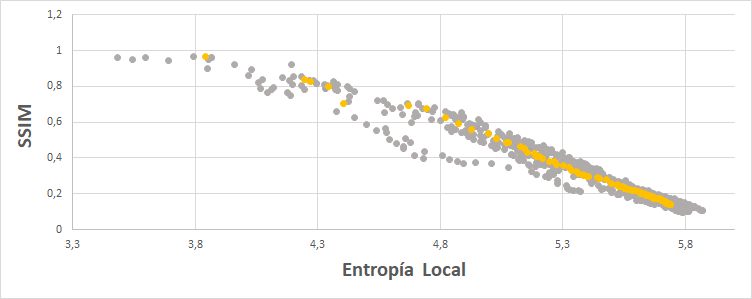
\includegraphics[width=14cm]{Chapter6/Chapter6Figs/FP-torax_frontal/img1-FP-variado-optimo.png}
    \caption {Resultados sub-óptimos obtenidos al aplicar los parámetros de optimización de la imagen \ref{fig:label:a} a las otras imágenes del mismo grupo (Tórax Frontal) \\
    {{\color{yellow} {$\bullet$}} Frente pareto óptimo}}
    \label{fp-original-resultante-tf}
  \end{center}
\end{figure}

En la \textbf{Figura \ref{fig:FP-robusto-sub-optimos}}, se comparan el Frente Pareto Robusto del grupo de imágenes de Tórax frontal y los Frentes Pareto sub-óptimos obtenidos por el proceso de prueba sobre todas las imágenes del grupo Tórax Frontal, utilizando las soluciones no dominadas de la imagen \textbf{\ref{fig:label:a}}, se puede observar que los resultados no son óptimos, pero son lo suficientemente válidos para el grupo de imágenes estudiados.

% Los parámetros que se obtuvieron en la Optimización Robusta son aplicables a cualquier imagen del grupo estudiado, a diferencia de trabajos anteriores, donde los parámetros se utilizaban para una sola imagen.

Además, se verifica que el Frente Pareto robusto cae en su óptimo con respecto a la optimización realizada sobre una sola imagen, pero en general se comporta de manera satisfactoria para el grupo de imágenes analizadas. Con esto también se observa que la solución óptima de una imagen $f$ no necesariamente es la mejor solución para una imagen $f_n$.

% %figuras FP entropia local/ssim tórax frontal imagen 2
\begin{figure}[H]
  \begin{center}
    \leavevmode
    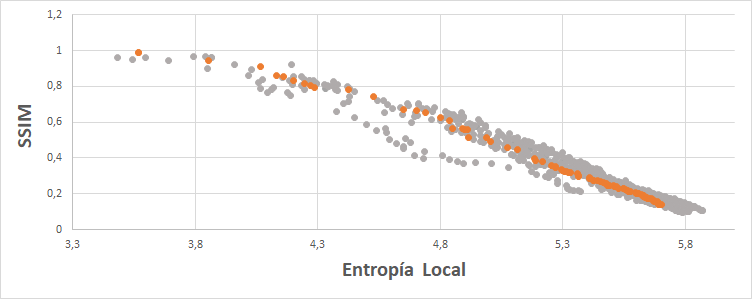
\includegraphics[width=14cm]{Chapter6/Chapter6Figs/FP-torax_frontal/img1-FP-variado-Frontal-robusto.png}
    \caption {Frente Pareto Entropía Local - SSIM. Tórax frontal\\}{
    Resultados sub-óptimos obtenidos al aplicar los parámetros de optimización de la imagen \ref{fig:label:a} a las otras imágenes del mismo grupo (Tórax Frontal).\\
    {{\color{myorange} {$\bullet$}} Frente pareto robusto}}
    \label{fig:FP-robusto-sub-optimos}
  \end{center}
\end{figure}

\begin{figure}[H]
  \begin{center}
    \leavevmode
    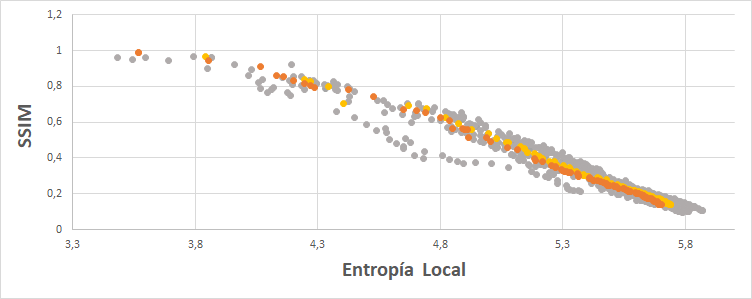
\includegraphics[width=14cm]{Chapter6/Chapter6Figs/FP-torax_frontal/img1-FP-variado-optimo-robusto.png}
    \caption {Frente Pareto Entropía Local - SSIM. Tórax frontal\\}{
    Resultados sub-óptimos obtenidos al aplicar los parámetros de optimización de la imagen \ref{fig:label:a} a las otras imágenes del mismo grupo (Tórax Frontal).\\
    {{\color{myorange} {$\bullet$}} Frente pareto robusto} \\
    {{\color{yellow} {$\bullet$}} Frente pareto óptimo}}
    \label{fig:FP-robusto-sub-optimos-optimo}
  \end{center}
\end{figure}


Para evaluar los resultados del Conjunto Pareto se utilizó la medición del hipervolumen \cite{hypervolume}. Esta métrica mide el área (2 objetivos) del espacio objetivo que es cubierto por el conjunto de soluciones, que está limitado por un punto de referencia. Esto equivale a la suma de todas las areas rectangulares, delimitadas por un punto de referencia. {\it yref}.

Cuando más grande es el valor del hipervolumen, se dice que es más dominante el conjunto de puntos del Frente Pareto. Esto hace que el hipervolumen sea una medida razonable para medir que tan eficiente es un Frente Pareto \cite{shah2016pareto}.

Para el punto de referencia se optó por el punto [6,1].

En la \textbf{Tablas \ref{tabla:hipervolumen-robustos} y \ref{tabla:hipervolumen-promedio-optimo}} se puede ver que el Hipervolumen cubierto por el Frente Pareto Robusto es similar al Hipervolumen cubierto por los Frentes Paretos Óptimos de las imágenes; es decir, el Frente Pareto Robusto no se encuentra muy lejos de los Frentes Paretos Óptimos. 
\begin{table}[H]
\centering
\caption{Hipervolumen de los Frentes Paretos Robustos.}
\begin{tabular}{|c|c|}
\hline
Frente Pareto Robusto & Valor Hipervolumen {\it yref}: [6,1] \\
\hline \hline 
\it{Tórax Frontal} & 0.99871 \\ \hline
\it{Tórax Lateral}  & 1.51317\\ \hline
\end{tabular}
\label{tabla:hipervolumen-robustos}
\end{table}

\begin{table}[H]
\centering
\caption{Hipervolumen promediado de los Frentes Paretos Óptimos.}
\begin{tabular}{|c|c|}
\hline
Frente Pareto Óptimo & Valor Hipervolumen {\it yref}: [6,1] \\
\hline \hline 
\it{Grupo Tórax Frontal} & 0,94578 \\ \hline
\it{Grupo Tórax Lateral}  & 1,45684\\ \hline
\end{tabular}
\label{tabla:hipervolumen-promedio-optimo}
\end{table}